
%----------------------------------------------------------------------------------------
%	PACKAGES AND OTHER DOCUMENT CONFIGURATIONS
%----------------------------------------------------------------------------------------

\documentclass{article}

\usepackage{fancyhdr} % Required for custom headers
\usepackage{lastpage} % Required to determine the last page for the footer
\usepackage{extramarks} % Required for headers and footers
\usepackage{graphicx} % Required to insert images
\usepackage{mathtools, bm}
\usepackage{amssymb, bm}
\usepackage{graphicx}
\usepackage{algorithmic}

% Margins
\topmargin=-0.45in
\evensidemargin=0in
\oddsidemargin=0in
\textwidth=6.5in
\textheight=9.0in
\headsep=0.25in


\linespread{1.1} % Line spacing

% Set up the header and footer
\pagestyle{fancy}
\lhead{\hmwkAuthorName} % Top left header
\chead{\hmwkClass\ (\hmwkClassInstructor\ \hmwkClassTime): \hmwkTitle} % Top center header
\rhead{\firstxmark} % Top right header
\lfoot{\lastxmark} % Bottom left footer
\cfoot{} % Bottom center footer
\rfoot{Page\ \thepage\ of\ \pageref{LastPage}} % Bottom right footer
\renewcommand\headrulewidth{0.4pt} % Size of the header rule
\renewcommand\footrulewidth{0.4pt} % Size of the footer rule

\setlength\parindent{0pt} % Removes all indentation from paragraphs

%----------------------------------------------------------------------------------------
%	DOCUMENT STRUCTURE COMMANDS
%	Skip this unless you know what you're doing
%----------------------------------------------------------------------------------------

% Header and footer for when a page split occurs within a problem environment


% Header and footer for when a page split occurs between problem environments
   
%----------------------------------------------------------------------------------------
%	NAME AND CLASS SECTION
%----------------------------------------------------------------------------------------
\newcommand{\logoepfl}{
  \begin{center}
    
\includegraphics[width=4cm]{img/epfl.jpg}
  \end{center}
  \vspace{0.3cm}
  \hrule
}


\newcommand{\hmwkTitle}{Decentralized Data Sharing System based on Secure Multiparty Computation} % Assignment title
\newcommand{\hmwkDueDate}{Autumn 2017} % Due date
\newcommand{\hmwkClass}{IN, LCA1} % Course/class
\newcommand{\hmwkClassTime}{} % Class/lecture time
\newcommand{\hmwkClassInstructor}{D.Froelicher, J.Troncoso-Pastoriza} % Teacher/lecturer
\newcommand{\hmwkAuthorName}{Max Premi} % Your name

%----------------------------------------------------------------------------------------
%	TITLE PAGE
%----------------------------------------------------------------------------------------
\title{
\logoepfl
\vspace{2in}
\textmd{\textbf{\hmwkClass:\ \hmwkTitle}}\\
\normalsize\vspace{0.1in}\small{Due\ on\ \hmwkDueDate}\\
\vspace{0.1in}\large{\textit{\hmwkClassInstructor\ \hmwkClassTime}}
\author{\textbf{\hmwkAuthorName}}
\vspace{3in}
}

%----------------------------------------------------------------------------------------

\begin{document}

\maketitle

\newpage
\section*{Abstract}
\addcontentsline{toc}{section}{Abstract}
Unlynx and Prio are two privacy-preserving data sharing systems, with each it's way to encode, decode and aggregate datas. While Unlynx uses homomorphic encryption based on Elliptic Curves and zero knowledge proofs, Prio uses Secret-sharing encoding and \textit{secret-shared non-interactive proofs}(SNIP's), which should perform much better in term of computation time, by doing more exchange between servers.\\
We consider $m$ servers that consitute the collective authority whose goal is to verifiably compute aggregation functions over data send by $n$ data providers.\\
Moreover, privacy is assured if at least one client is trusted, and it then assure  robustness and scalability,  with several other mechanics such as Noise addition for Unlynx or SNIPs proof for Prio. In both case the number of servers should be significantly smaller than the number of client.\\
Prio also extends classic private aggregation techniques to enable collection of different class of statistics such as least-square regression.\\
This paper presents the implementation of Prio aggregation system and input proof into Unlynx, as well as an input validation proof for Unlynx Aggregation system, and then compare both of those to see which one scale better.
%----------------------------------------------------------------------------------------
%	TABLE OF CONTENTS
%----------------------------------------------------------------------------------------

\newpage
\tableofcontents
\newpage


%----------------------------------------------------------------------------------------
%	BEGIN OF REPORT
%----------------------------------------------------------------------------------------

\section*{Introduction}
\addcontentsline{toc}{section}{Introduction}
Nowadays, tons of data are generated around us and about what we do, and are used to compute statistics. Even if these statistics are colleted with the goal of learning usefull aggregate informations about the users/population, it might collect and store private data from client.\\
The need of collecting data and sharing them in a privacy-preserving way has become crucial in this context. A lot of techniques have been developed through the years, by major technology companies such as Google [references], but also researcher in Universities [references].\\
\begin{itemize}
\item \textbf{Put some example applications}\\
\end{itemize}
However, by gaining \textit{privacy}, these protocols sacrifice \textit{robustness} and \textit{scalability},\\
\begin{itemize}
\item \textbf{Explain the link between the two and why}
\end{itemize}
, leading to the use of technical agreements rather than technical solutions.\\
In this paper, we present the implementation of Prio into Unlynx and compare them with input validation proof.

\section*{Contributions}
\section*{Background}

\section{Unlynx System}
\begin{itemize}
\item How does unlynx work (with a figure) (system of client, queries and servers)
\item How Aggregation is done
\item How proof is done
\end{itemize}
\subsection{Model}
Unlynx is a privacy-preserving data sharing system developed by LCA1 in collaboration with DeDiS.\\
It consists of a collective authority (CA) formed by a number $m$ of server $S_1,...S_m$,and $n$ data providers $DP_1,...DP_n$. These DPs combined represent a distributed databased that is used to awnser queries made by a querier $Q$. The querier and DPs choose one server of the CA to communicate with and can change this choice at any given time.\\
\textbf{Functionality} Unlynx should permit SQL queries of the form SELECT SUM(*)/COUNT(*) FROM DP,.... WHERE * AND/OR GROUP BY *, with any number of * clauses.

\subsection{Threats}
\textbf{Collective authority servers} It is assumed an Anytrust model [REF]. It does not requires any particular server to be trusted or to be honest-but-curious. The moment it exists one server that is not malicious, functionality, security and privacy are guaranteed.\\
\textbf{Data providers} are assumed to be honest-but-curious. The system does not protect against malicious DPs sending false infomations, but a solution will be discuss  in Section [INPUT RANGE VALID SECTION].\\
\textbf{Queriers} are assumed to be malicious, and can collude between themselves or with a subset of the CA servers.\\
It is also assumed tha all network communication is encrypted and authenticated, by using TLS.

\subsection{Pipeline and proof}
The protocol start when a querier wants to retrieve some information about sensitive data. It sends the query to one of the server of the CA. Upon receiving, the server broadcast this query to the other servers in the collective authority.\\
From here the data are privately and securely processed by the CA, before sending back the result to the querier.\\
The pipeline is the following: Encryption, Verification Shuffle, Distributed Deterministig Tag, Collective Aggregation, Distributed Results Obfuscation, Key Switch. At the end of this pipeline, the querier get the data and can decrypt them to get the aggregate data he asked, without any server seeing the data in clear, or knowing from which data provider the data are from.
\begin{figure}[h]
\centering
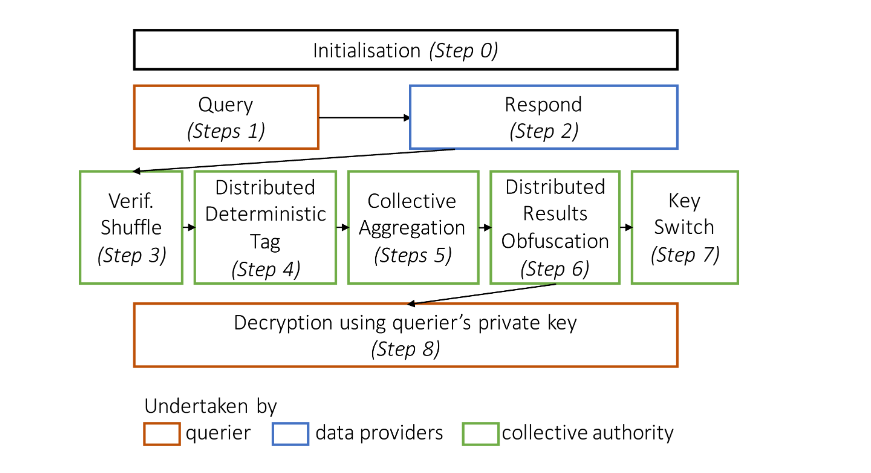
\includegraphics[scale=0.5]{img/unlynxPip.png}
\caption{Unlynx query processing pipeline}
\end{figure}
\\
\textbf{Proofs} are done with zero-knowledge systems, to preserve privacy. There is one for each state of the pipeline, for example when aggregating, it publishes the result of the local aggregation, as the data is encrypted using ElGamal Elliptic curves, it leaks nothing about the data alone, but there is no Input range proof , meaning the DPs can send fraudulous data (by giving a very big number, and as it is encoded we cannot verify it) and make the computation wrong. This is implemented and described in section [SECTION]\\

\section{Prio System}
\begin{itemize}
\item How does Prio work (same as before)
\item How does Aggregation is done
\item New proof system SNIPs
\end{itemize}
\subsection{Model}
Prio is also a privacy-preserving sharing sytem, where each DPs holds a private value $x_i$. The goal of the CA is to compute an aggregation function $f(x_1,...x_n)$, in a way that leaks as little as possible about each $x_i$ values to the server. Unlike Unlynx, Prio do not encrypt private value $x_i$ that why it is a more challenging aggregation in terms of privacy.\\
As Unlynx communication is assumed to be done in secure channels. Privacy is assured as long as one server is trusted and correctness is provided if and only if all server are honest.

\subsection{Threats}
do

\subsection{Pipeline and proof}
do 
\section*{Prio SNIPs}
\begin{itemize}
\item Client evaluation
\item Consistency checking at the server
\item Polynomial identity test
\item Multiplication of shares
\item Output verification

\end{itemize}

\subsection{Input range validation for ElGamal}
do

\section*{Implementation}
\begin{itemize}

\item what is implemented in a little more detailled
\item optimization apported by code from github and not aborded in details

\end{itemize}
\section*{Performance evaluation}

Explain a little more about comparison and test settings


\begin{itemize}


\item Scaling with number of server
\item Scaling with number of client
\item Scaling with fairly high number of both 
\item Time and Bandwidth dilemna

\end{itemize}
\section*{El Gamal range input checking}
\begin{itemize}

\item TO be seen
\end{itemize}
\appendix
\newpage

\newpage
\section*{Conclusion}
\addcontentsline{toc}{section}{Conclusion}

\newpage
\section*{References}
\addcontentsline{toc}{section}{References}


\end{document}
